\section{Implementation}
\label{sec:implementation}

This section describes the languages and platforms on which Zeroties is based.
It then illustrates the different components in Zeroties: the daemon, the browser addon, and the communication between these components.

\subsection{Languages and Platforms}
\label{sub:languages_and_platforms}

All components are written in JavaScript. 
The Zeroties daemon is written using Node.js\footnote{https://nodejs.org/en/, accessed 2019-04-17}, the browser addons are written with the vendor-specific addon frameworks.
We decided on JavaScript for all components due to several reasons:
\begin{itemize}
\item We wanted the OS-level Zeroties daemon to be as platform-independent as possible. 
Node.js is a stable environment on all major operating systems by now.
\item We wanted to lean on a library implementing the low-level Zeroconf protocols.
We found a capable, mature, and well-maintained library, \textit{dnssd}\footnote{https://www.npmjs.com/package/dnssd, accessed 2019-04-17} available for this purpose on Node.js.
\item Browser addons must be implemented in JavaScript.
Despite the fact that we could not integrate the core Zeroties functionality into our browser addons (see Section~\ref{sec:approach}) we still wanted to avoid  introducing a language barrier that would prevent us to do so even without browser-specific restrictions.
\item Starting a HTTP server and a WebSocket server in Node.js and connecting to these servers from an addon is inherently straight-forward.
This functionality was required for our purpose.
\end{itemize}

\subsection{Zeroties Daemon}
\label{sub:zeroties_daemon}

At the core of Zeroties is the Zeroties daemon.
This is the piece of software that any application wishing to make use of the Zeroties services must connect to.
The daemon runs continuously in the background on the user's operating system with a server to handle interactions with Zeroties applications.
Zeroties applications are provided the following two pieces of core functionality by interacting with the Zeroties daemon:
\begin{itemize}
    \item The ability to publish services on the local network, via mDNS.
    \item Notifications when the list of services available on the local network changes, as discovered via DNSSD.
\end{itemize}
The Zeroties daemon is also responsible for handling any client HTTP request or WebSocket connection to the server published by a Zeroties application.
Instead of handling these events directly, the daemon acts as a proxy, forwarding the events to the Zeroties app as approriate.
This allows developers of Zeroties applications to easily define custom routing for HTTP requests recieved, and define custom actions to handle different WebSocket events.

All communication between Zeroties applications and the Zeroties daemon is made via a WebSocket connection, following the protocol outlined as follows: on connecting to the daemon, applications are automatically subscribed to recieve notifications about changes to the list of available Zeroties services.
The daemon repeatedly polls the network to retrieve the current list of Zeroties services using the DNSSD protocol.
If the list of services retrieved from the network differs from the one currently held by the daemon, an event is triggered.
This event is fired over the WebSocket connection to all listening Zeroties applications.
To publish a service, a Zeroties application sends a message to the daemon containing the name of the service to publish.
The Zeroties daemon then spins up an HTTP server and a WebSocket server listening on the same port, and advertises the newly available service over the local network via mDNS.


% what it is:
% - the core Zeroties daemon
% - any application wishing to use Zeroties must communicate with this app

% what does it do:
% - facilitates publishing services on the local network
% - notifies clients on updates to available services list
% - handles client connections and forwards requests/messages to Zeroties app for handling (acts as a proxy)


% how does it work:
% - services list is maintained/updated via mdns/dnssd
% - Zeroties apps connect to the Zeroties daemon via a Websocket connection
% - on connecting, clients are automatically subscribed to recieve updates about changes to the list of services
% - Zeroties apps notify the Zeroties daemon if they wish to publish a server
% - clients connect to Zeroties daemon server
% - server forwards to Zeroties app for handling via websockets
% - Websocket communication allows us to define http request handling behaviour in the browser
% - request/response protocol

% could it be improved?:


\textbf{Zeroties Communication Protocol.} Communication with the Zeroties daemon must follow a certain protocol.

\begin{itemize}
\item \textit{Messages to the Zeroties Daemon}: at the moment, there is only one supported message that may be sent to the Zeroties Daemon unprompted: the \texttt{publish} message.
The message must send a JSON string of the following format: 
\begin{lstlisting}[breaklines]
{method: "publish", payload: {name: appName}}
\end{lstlisting}
This is the message that informs the Zeroties daemon that the application wishes to publish a service.
\item \textit{Messages from the Zeroties Daemon}: any app connected to the Zeroties daemon should expect to receive and handle a message in the following format:
\begin{lstlisting}[breaklines]
{method: "servicesChanged", services: <array of services>}
\end{lstlisting}
This is the message sent by the Zeroties daemon whenever a change in the list of Zeroties services is detected.
Table~\ref{tab:zeroties_protocol} outlines the messages sent from the Zeroties daemon sent to its applications that publish a service, as well as the expected responses to these messages.
\end{itemize}


\begin{table*}[h]
\small
\centering
\caption{The messages sent to Zeroties apps by the Zeroties daemon, and the responses which are expected back. After recieving a \texttt{wsForwardResponse}, the daemon will respond again with a \texttt{wsProxyHandshake} message.}
\def\arraystretch{2}
\begin{tabularx}{\textwidth}{l|l|l|l}
\textbf{Method} & \textbf{Response} & \textbf{Response to response} & \textbf{\pbox{9.5cm}{Purpose}}\\
\hline
\texttt{request} & \texttt{response} & & \pbox{9.5cm}{Dispatches an incoming HTTP request to the Zeroties App for handling. Waits for a response containing the serialized response}\\ \hline
\texttt{wsForward} & \texttt{wsForwardResponse} & \texttt{wsProxyHandshake} & \pbox{9.5cm}{Notifies the Zeroties app of an incoming WebSocket connection and establishes a proxy connection}\\ \hline
\texttt{wsForward} & \texttt{init} & & \pbox{9.5cm}{To complete the proxy connection, the Zeroties app must send an init message over the proxy connection once it is open}\\
\end{tabularx}
\label{tab:zeroties_protocol}
\end{table*}

\subsection{Browser Addons}
\label{sub:browser_addons}

The Zeroties browser addon is an intermediary layer that easily allows web applications to function as Zeroties apps.
They expose a simple API that abstracts away the underlying complexities of proxy communication with the Zeroties server.
The addon works by injecting the API script into all accessed webpages using a content script.

\textbf{API for web applications.}
The Zeroties addon API consists of two functions:
\begin{itemize}
\item \texttt{navigator.publishServer(appName)} sends a message to the Zeroties daemon, which then attempts to publish a server with the specified name.
It returns a Promise, which resolves to a server object. 
From this server object, behaviour for handling HTTP requests and WebSockets can be defined.
\item \texttt{window.addEventListener("zerotiesServicesChanged", callback)} listens for the  \texttt{zerotiesServicesChanged} event. This event is triggered by the Zeroties daemon whenever the list of Zeroties services available has changed.
The second parameter is a callback function which recieves the updated services list as its argument.
\end{itemize}

This API roughly mimicks the one that was provided by FlyWeb, so migrating a (Successorships-)FlyWeb application to Zeroties involves only minimal changes\footnote{Obviously, we did not want to keep the name \texttt{flywebServicesChanged} for our event.}.

The Zeroties addon also contains a browser menu button that renders a popup upon click showing a list of currently available services.
This list is updated live through the WebSocket channel to the Zeroties daemon.
Figure~\ref{fig:addon} shows a screenshot of this popup with a single service being published.
A click on a service in this list will open a new tab and connect to the service as a client.

\begin{figure}[h]
    \centering
    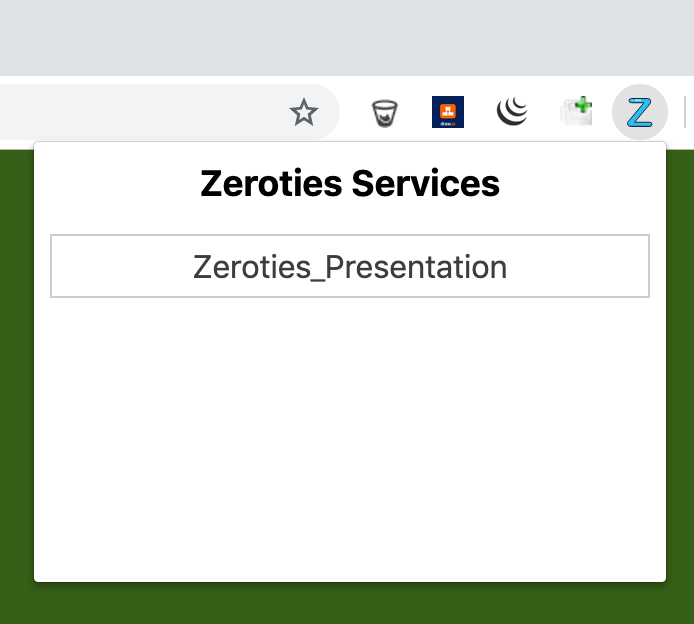
\includegraphics[keepaspectratio,width=6cm]{addon}
    \caption{Addon services menu.}
    \label{fig:addon}
\end{figure}

% what is it:
% - addons for chrome and firefox
% - an example of a Zeroties app

% what does it do:
% - provides a simple interface to webapps for communcation with the Zeroties daemon
% - abstracts away all the websocket nonsense
% - popup shows all published zeroties services on the local network

% how does it work:
% - communicates with the Zeroties daemon via websockets following request/response protocol
% - injects a script to webapps which exposes the api via window/navigator

\subsection{Communication and Control Flow in Zeroties}
\label{sub:communication}

This section discusses the flow of control and the communication between Zeroties apps and the Zeroties daemon, using Successorships as an example.
Listing~\ref{lst:publish_service} shows an example usage of the \texttt{publishServer} API.
The functions \texttt{onFetch}, \texttt{onWebsocket}, and \texttt{onClose} are event listeners that are called when their respective events are dispatched.

\begin{lstlisting}[caption={Publishing of a service},label={lst:publish_service}]
navigator.publishServer(Shippy.internal.appName()).then(function(server) {
  // ...
  server.onfetch = onFetch;
  server.onwebsocket = onWebsocket;
  server.onclose = onClose;
  // ...
}).catch(function (err) {
  // ...
});
\end{lstlisting}

When the \texttt{onWebsocket} function is called, a WebSocket connection with the Zeroties daemon is established.
This WebSocket serves as the main channel of communication between the daemon and the addon, which interacts directly with the web application.
Whenever a client triggers an event on the published server, for example upon recieving an HTTP request, it is forwarded to the addon via a WebSocket message.
In the case of an HTTP request, the \texttt{onFetch} function is called, which generates a response to the request.
The response is then serialized and sent back over the WebSocket as the payload of another message.
Finally, the response is deserialized by the Zeroties daemon and dispatched back to the appropriate client.
To make sure responses are sent back to the correct client, all messages in this series of events are accompanied by a unique identifier that is generated when the HTTP request is first recieved.

WebSocket connection events follow a similar control pattern.
When the published server recives a WebSocket connection, the Zeroties daemon notifies the addon of the new connection with a WebSocket message.
The addon then creates a new WebSocket connection with the daemon. 
This means that for each client connected to the server, there is a proxy WebSocket between the daemon and the addon.
This facilitates pseudo-direct communication between the server webapp and its clients.
WebSocket messages are sent from the client to the published server, and then forwarded by the daemon over the proxy connection to the server webapp.
The reverse is true for messages sent from the server webapp to the client.

Listing~\ref{lst:service_discovery} shows an example of subscribing to changes in the Zeroties services list.
This is a fairly straightforward process: the Zeroties daemon polls the network for changes in the services list using DNSSD.

\begin{lstlisting}[caption={Service discovery},label={lst:service_discovery}]
window.addEventListener('zerotiesServicesChanged', function (event) {
  // ...
});
\end{lstlisting}

When a change is detected, the daemon sends a message over the WebSocket connection to the addon.
This message contains the updated services list.
The addon then dispatches a \texttt{zerotiesServicesChanged} event on the global \texttt{window} object with the updated services list as payload.
